
%%%%%%
%
% $Autor: Wings $
% $Datum: 2020-01-18 11:15:45Z $
% $Pfad: WuSt/Skript/Produktspezifikation/powerpoint/ImageProcessing.tex $
% $Version: 4620 $
%
%%%%%%

\chapter{Zeichnungen mit tikz}


Das Paket tikz ist ein mächtiges Werkzeug zu erstellen von Grafiken. Es existieren vielen Einführungen. Hier werden nur die ersten Schritte gezeigt, so dass man leicht Flussdiagramme erzeugen kann.

\bigskip

Zeichnen einer Linie und Pfeile

\lstinputlisting{tikz/Line.tex}

\medskip

\begin{tikzpicture}
    \draw (0,0) -- (1,0);
    
    \draw[->] (2,0) -- (3,0);

    \draw[<->] (5,0) -- (6,0);
\end{tikzpicture}

\bigskip

Zeichnen einer dicken, blauen Linie

\lstinputlisting{tikz/Line2.tex}

\medskip

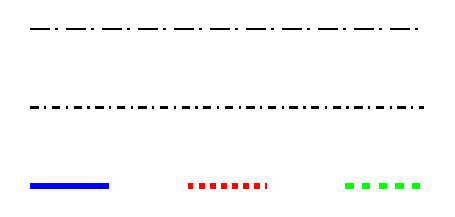
\begin{tikzpicture}
    \draw[line width=2pt, blue] (0,0) -- (1,0);

    \draw[line width=2pt, red, dotted] (2,0) -- (3,0);

    \draw[line width=2pt, dashed, green] (4,0) -- (5,0);

    \draw [thick,dash dot] (0,1) -- (5,1);  
    \draw [thick,dash pattern={on 7pt off 2pt on 1pt off 3pt}] (0,2) -- (5,2);
\end{tikzpicture}

\bigskip

Zeichnen eines Kreisbogens

\lstinputlisting{tikz/arc.tex}

\medskip

\input{tikz/arc.tex}

\bigskip

Zeichnen einer Funktion

\lstinputlisting{tikz/function.tex}

\medskip

\input{tikz/function.tex}

\bigskip

Zeichnen von Rechtecken und Verschiebung von Objekten

\lstinputlisting{tikz/rectangle.tex}

\medskip

\input{tikz/rectangle.tex}

\bigskip

%Einbringen von Text left right bottom top

\bigskip

Verwendung von Variablen

\lstinputlisting{tikz/variable.tex}

\medskip

\input{tikz/variable.tex}

\bigskip

Verwendung von Punkten

\lstinputlisting{tikz/node.tex}

\medskip

\input{tikz/node.tex}

\bigskip
Verwendung von Punkten

\lstinputlisting{tikz/node3.tex}

\medskip

\input{tikz/node3.tex}

\bigskip
Verwendung von Punkten

\lstinputlisting{tikz/node2.tex}

\medskip

\input{tikz/node2.tex}
